%%%%%%%%%%%%%%%%%%%%%%%%%%%%%%%%%%%%%%%%%%%%%%%%%%%%%%%%%%%%%%%%%%%%%%%%%%%%%%%%
% Set Alarm
%%%%%%%%%%%%%%%%%%%%%%%%%%%%%%%%%%%%%%%%%%%%%%%%%%%%%%%%%%%%%%%%%%%%%%%%%%%%%%%%
\chapter{Set Alarm} \label{Set Alarm}
\vspace{-10ex}\mSA{syml}\vskip 8ex

%%%%%%%%%%%%%%%%%%%%%%%%%%%%%%%%%%%%%%%%%%%%%%%%%%%%%%%%%%%%%%%%%%%%%%%%%%%%%%%%
% Introduction
%%%%%%%%%%%%%%%%%%%%%%%%%%%%%%%%%%%%%%%%%%%%%%%%%%%%%%%%%%%%%%%%%%%%%%%%%%%%%%%%
\section{Introduction}

Allows setting a \textit{time of day} alarm where either the \cBe{f} or
\mAu{f} can be used as an alarm wakeup source.  Additionally it allows for
setting the amount of time the alarm will snooze as well as automatic off times
for when the alarm has been alerting or \sAlIP{f} for too long.  The time will
be displayed in either \num{12} or \num{24} hour format, whichever is used to
display the \mCl{f}.

\par\medskip

It is the \mPr{f} mode when the \cRs{f} is in the \dLe{f}
position.  See \hyperref[Alarm]{\mAl{f}} for more information on how the alarm
functions.

\par\medskip

There are a few ways to get to \mSA{f} depending on which direction the \cRs{f}
is pointing and which mode the device is currently in.

\begin{table}[H]
\ers{3}
\centering
\begin{tabu} { X[1,c,m] | X[1,c,m] | X[1,c,m] }
  \thrule
  \thbi{Position} & \thbi{Mode} & \thbi{Action} \\ \mrule

  \sMi & \multirow{2}{*}[-1mm]{\mode{s}{ANY}}
    & $\hskip -5mm$ \sMtoL \\ \dcrule{1}{1} \dcrule{3}{3}
  \sRi & & \sRtoL \\ \mdrule

  \multirow{4}{*}[-1.5mm]{\sLe}
    & \mSC{sym} & \sSec \\ \dcrule{2}{3}

  & \multirow{2}{*}[-1.5mm]{\mTS{sym}}
    & \sSec \\ \dcrule{3}{3}

  & & \sTer \\ \dcrule{2}{3}

  & \mode{f}{ANY} & \sLtoM \quad\quad \sMtoL \\

  \bhrule
\end{tabu}
\caption{Set Alarm - Mode}
\end{table}

\pagebreak

A few items of note:

\begin{itemize}
  \item All previously saved settings will initially be loaded.
  \item After setting the time of day, you can change mode and the settings
    will be saved and the \mAl{f} will be set.  This allows for setting the time
    without having to go through the rest of the settings.
  \item To \aReset{f}, \aPH{f} the \cEs{f} until \symD{<<<<} is blinking on
    the \cDi{f}.
    \begin{enumerate}
      \item If \aReset{f} from the \sSAHo{f} state, the alarm will be
        \sSADi{f} and display \symD{OFF!}.
      \item From any other state, it will start over from the \sSAHo{f} state.
    \end{enumerate}
  \item When the alarm is \sSADi{f}, \aPR{f} the \cEs{f} to enable the alarm.
\end{itemize}

%%%%%%%%%%%%%%%%%%%%%%%%%%%%%%%%%%%%%%%%%%%%%%%%%%%%%%%%%%%%%%%%%%%%%%%%%%%%%%%%
% Overview
%%%%%%%%%%%%%%%%%%%%%%%%%%%%%%%%%%%%%%%%%%%%%%%%%%%%%%%%%%%%%%%%%%%%%%%%%%%%%%%%
\section{Overview}

There are a number of states \mSA{f} can be in and are explained in the next
sections.

\begin{table}[H]
\ers{2}
\centering
\begin{tabu}{ X[1,c,m] | X[3,l,m] }
  \thrule

  \thbi{State} & \thbi{Description} \\ \mrule

  \sSAHo{sym} & Set the hour. \\ \drule{2}
  \sSAMi{sym} & Set the minute. \\ \drule{2}
  \sSAWS{sym} & Set the wakeup source - either \cBe{f} or \mAu{f}. \\ \drule{2}
  \sSAST{sym} & Set the amount of time the alarm will snooze. \\ \drule{2}
  \sSAWT{sym} & Set the amount of time the alarm can be alerting, i.e. in the
    \sAlWa{f} state, before automatically turning off. \\ \drule{2}
  \sSATT{sym} & Set the amount of time the alarm can be \sAlIP{f} 
                before automatically turning off. \\ \drule{2}
  \sSADo{sym} & Display alarm settings. \\ \drule{2}
  \sSADi{sym} & Alarm is disabled. \\
  \bhrule
\end{tabu}
\caption{Set Alarm - States}
\end{table}

\mSA{f} will initially start out in one of two states - \sSAHo{f} or \sSADi{f}.
If the alarm is \sSADi{f}, the display will show

\begin{figure}[H]
\centering
  \sDl{OFF!}
\end{figure}

and it will \textit{not} be blinking.  To enable the alarm, \aPR{f} the \cEs{f}.

\as{{c c c c}}{\sSADi{sym} & \sPR & \eEn{sym}{ALARM} & \sSAHo{sym} \\}

After being enabled, any previously saved settings will be in effect so you
do not need to reconfigure the alarm unless you want to change it.

\par\medskip

If you want to disable the alarm, from \sSAHo{f}, perform a \aReset{f}, i.e.
\aPH{f} the \cEs{f} until \symD{<<<<} is blinking on the display then \aRe{f}.

\as{{c c c c}}{\sSAHo{sym} & \sReset & \eDisable{sym}{ALARM} & \sSADi{sym} \\}

\info{The alarm can only be \sSADi{f} from the \sSAHo{f} state.  A \aReset{f} from
any other state will start over from the \sSAHo{f} state.}

\par\medskip

When enabled, to progress through the states, you will \aTu{f} the
\cEs{f} to select a value, then \aPR{f} the \cEs{f} to cache the setting and
move on to the next setting.

\tabcolsep=8pt
\as{{ c c c c c c c c c c c c c }}{%
\sSAHo{sym} & \sTu & \sPR & \sSAMi{sym} & \sTu & \sPR
  & \sSAWS{sym} & \sTu & \sPR & $\cdots$\quad$\cdots$
    & \sSADo{sym} & \sPR & \sSAHo{sym} \\}
\tabcolsep=12pt

When all settings have been configured, the \sSADo{f} state cycles through and
displays each one.  It will cycle repeatedly until you \aPR{f} the \cEs{f}.

\par\medskip

After setting and caching the \sSAMi{f}, you can short circuit the process by
changing mode and the alarm will be set and saved.

\tabcolsep=10pt
\ase{3}{{m{4.1in} m{0.8in} m{0.8in} m{1mm}}}{%
  \begin{tabu}{c c c c c c c}
    \sSAHo{sym} & \sTu & \sPR & \sSAMi{sym} & \sTu & \sPR & \sSAWS{sym}
  \end{tabu} &
  \begin{tabu}{c}
    \sSec \\ \drule{1} \sTer \\ \drule{1} $\hskip -5.5mm$ \sLtoM \\ \drule{1} \sLtoR
  \end{tabu} &
  {\ers{0.1} \begin{tabu}{c} \eSe{sym}{ALARM} \\ \eSa{sym}{ALARM} \end{tabu}} & \\}
\tabcolsep=12pt

%%%%%%%%%%%%%%%%%%%%%%%%%%%%%%%%%%%%%%%%%%%%%%%%%%%%%%%%%%%%%%%%%%%%%%%%%%%%%%%%
% Time
%%%%%%%%%%%%%%%%%%%%%%%%%%%%%%%%%%%%%%%%%%%%%%%%%%%%%%%%%%%%%%%%%%%%%%%%%%%%%%%%
\pagebreak
\section{Time} \label{Set Alarm - Time}

Setting the alarm \textit{time of day} happens on one screen of the \cDi{f} and
is composed of two states - \sSAHo{f} and \sSAMi{f}. The current setting, first
\sSAHo{f}, then \sSAMi{f}, will be \textit{blinking}.  The time will be
displayed in the current format that was chosen in \hyperref[Set Clock]{\mSC{f}}.

\par\medskip

For \num{12} hour format, a \textit{decimal} at the \textit{lower right} of the
\cDi{f} is the \mono{PM} indicator.

\figDT{11:00}{11 AM}{11:00.}{11 PM}

A couple of examples in \num{12} and \num{24} hour format:

\begin{table}[H]
\ers{2.5}
\begin{tabu}{X[2,l,m] | X[1,c,m] | X[1,c,m]}
  \thrule
  & \thbi{12 Hour} & \thbi{24 Hour} \\ \mrule
  Seven in the Morning & \sDl{!7:00} & \sDl{07:00} \\ \drule{3}
  Seven (or 19:00) in the Evening & \sDl{!7:00.} & \sDl{19:00} \\
  \bhrule
\end{tabu}
\end{table}

%%%%%%%%%%%%%%%%%%%%%%%%%%%%%%%%%%%%%%%%%%%%%%%%%%%%%%%%%%%%%%%%%%%%%%%%%%%%%%%%
% Time - Hour
%%%%%%%%%%%%%%%%%%%%%%%%%%%%%%%%%%%%%%%%%%%%%%%%%%%%%%%%%%%%%%%%%%%%%%%%%%%%%%%%
\subsection{Hour} \sSAHo{syml}

Set the hour when the alarm will start.

\par\medskip

To select the \sSAHo{f}, \aTu{f} the \cEs{f} then \aPR{f} to cache the setting and
move on to \sSAMi{f}.

\as{{c c c c}}{%
\multirow{2}{*}{\sSAHo{sym}}
  & \sTu & \sPR & \multirow{2}{*}{\sSAMi{sym}} \\
& \eUp{sym}{} & \eCa{sym}{} & \\}

You can turn in either direction to get to the hour you want to set.  The hour
will wrap at the \num{0} and \num{23} hour marks if the current format is
\num{24} hour.

\begin{table}[H]
\ers{1}
\centering
\begin{tabu} { c c c }
  \mrule
  \sD{00:00} & \sCC & \sD{23:00} \\
  \mrule
\end{tabu}
\quad\quad\quad\quad
\begin{tabu} { c c c }
  \mrule
  \sD{23:00} & \sCl & \sD{00:00} \\
  \mrule
\end{tabu}
\end{table}

For \num{12} hour format, the transitions between \mono{AM} and \mono{PM} when
turning clockwise and counter-clockwise from \num{12} \mono{AM} back to
\num{12} \mono{AM} are shown below.

\ase{1}{{ c c c c c c c c}}{%
\sCl & \sD{12:00} & $\cdots$ & \sD{11:00} & \sD{12:00.}
  & $\cdots$ & \sD{11:00.} & \sD{12:00} \\ \drule{8}
\sCC & \sD{12:00} & \sD{11:00.} & $\cdots$ & \sD{12:00.}
  & \sD{11:00} & $\cdots$ & \sD{12:00} \\}

%%%%%%%%%%%%%%%%%%%%%%%%%%%%%%%%%%%%%%%%%%%%%%%%%%%%%%%%%%%%%%%%%%%%%%%%%%%%%%%%
% Time - Minute
%%%%%%%%%%%%%%%%%%%%%%%%%%%%%%%%%%%%%%%%%%%%%%%%%%%%%%%%%%%%%%%%%%%%%%%%%%%%%%%%
\pagebreak
\subsection{Minute} \sSAMi{syml}

Set the minute when the alarm will start.

\par\medskip

To select the \sSAMi{f}, \aTu{f} the \cEs{f} then \aPR{f} to cache the setting and
move on to \sSAWS{f}.

\as{{c c c c }}{%
\multirow{2}{*}{\sSAMi{sym}}
  & \sTu & \sPR & \multirow{2}{*}{\sSAWS{sym}} \\
& \eUp{sym}{} & \eCa{sym}{} & \\}

\info{At this point, after caching, you can \aTu{f} the \cRs{f} or change mode
and the alarm will be set and saved.}

%%%%%%%%%%%%%%%%%%%%%%%%%%%%%%%%%%%%%%%%%%%%%%%%%%%%%%%%%%%%%%%%%%%%%%%%%%%%%%%%
% Wakeup Source
%%%%%%%%%%%%%%%%%%%%%%%%%%%%%%%%%%%%%%%%%%%%%%%%%%%%%%%%%%%%%%%%%%%%%%%%%%%%%%%%
\section{Wakeup Source} \sSAWS{syml}

Set the wakeup source when the alarm starts and wakes.

\par\medskip

Either the \cBe{f} or \mAu{f} can be chosen as a wakeup source when the alarm
starts or resumes from snoozing. 

\figDT{bEEP}{Wake to \cBe{ss}}{PLAY}{Wake to \mAu{ss}}

\info{%
If the \mAu{f} is \sAuOc{f} when the alarm starts, the \cBe{f}
will be used regardless of setting.
The \mAu{f} is considered \sAuOc{f} if either of the following are true:
\begin{itemize}
  \item \mAu{f} is in the \sAuPl{f} state, \textit{or}
  \item \cPl{f}, \cNe{f} or \cPr{f} push-buttons are being \action{f}{PRESSED}.
\end{itemize}}
To select the wakeup source, \aTu{f} the \cEs{f} then \aPR{f}
to cache the setting and move on to \sSAST{f}.

\as{{c c c c }}{%
\multirow{2}{*}{\sSAWS{sym}}
  & \sTu & \sPR & \multirow{2}{*}{\sSAST{sym}} \\
& \eUp{sym}{} & \eCa{sym}{} & \\}

%%%%%%%%%%%%%%%%%%%%%%%%%%%%%%%%%%%%%%%%%%%%%%%%%%%%%%%%%%%%%%%%%%%%%%%%%%%%%%%%
% Snooze Time
%%%%%%%%%%%%%%%%%%%%%%%%%%%%%%%%%%%%%%%%%%%%%%%%%%%%%%%%%%%%%%%%%%%%%%%%%%%%%%%%
\section{Snooze Time} \sSAST{syml}

Set the amount of time in \textit{minutes} the alarm will snooze.

\par\medskip

The \cDi{f} will show the following

\figD{Sn:10}{10 Minutes}

and the number on the \textit{right} side of the \textit{colon} will be
\textit{blinking}.  The time can be set from \num{1} to \num{59} minutes.

\par\medskip

To select the \sSAST{f} in minutes, \aTu{f} the \cEs{f} then \aPR{f}
to cache the setting and move on to \sSAWT{f}.

\as{{c c c c }}{%
\multirow{2}{*}{\sSAST{sym}}
  & \sTu & \sPR & \multirow{2}{*}{\sSAWT{sym}} \\
& \eUp{sym}{} & \eCa{sym}{} & \\}

%%%%%%%%%%%%%%%%%%%%%%%%%%%%%%%%%%%%%%%%%%%%%%%%%%%%%%%%%%%%%%%%%%%%%%%%%%%%%%%%
% Wake Time
%%%%%%%%%%%%%%%%%%%%%%%%%%%%%%%%%%%%%%%%%%%%%%%%%%%%%%%%%%%%%%%%%%%%%%%%%%%%%%%%
\section{Wake Time} \sSAWT{syml}

Set the amount of time in \textit{minutes} that the alarm can alert for, without
being snoozed or manually stopped, before automatically stopping the alarm.
Useful if you forget to stop the alarm so it doesn't beep or play music all day.

\info{%
Set to \num{0} to \action{f}{DISABLE} this setting - the alarm will
alert until manually snoozed, stopped or, if enabled, the \sSATT{f} is
exceeded.}

The \cDi{f} will show the following

\figDT{On:10}{10 Minutes}{On:!0}{Disabled}

and the number on the \textit{right} side of the \textit{colon} will be
\textit{blinking}.  The time can be set from
\num{0} to \num{59} minutes with the value \num{0} being \state{f}{DISABLED}.

\par\medskip

To select the \sSAWT{f} in minutes, \aTu{f} the \cEs{f} then \aPR{f}
to cache the setting and move on to \sSATT{f}.

\as{{c c c c }}{%
\multirow{2}{*}{\sSAWT{sym}}
  & \sTu & \sPR & \multirow{2}{*}{\sSATT{sym}} \\
& \eUp{sym}{} & \eCa{sym}{} & \\}

%%%%%%%%%%%%%%%%%%%%%%%%%%%%%%%%%%%%%%%%%%%%%%%%%%%%%%%%%%%%%%%%%%%%%%%%%%%%%%%%
% Total Alarm Time
%%%%%%%%%%%%%%%%%%%%%%%%%%%%%%%%%%%%%%%%%%%%%%%%%%%%%%%%%%%%%%%%%%%%%%%%%%%%%%%%
\section{Total Alarm Time} \sSATT{syml}

Set the total amount of time in \textit{hours} that the alarm can be active or
\sAlIP{f} for after starting before automatically stopping the alarm.
Useful if you just don't want to get up in the morning and would otherwise
indefinitely snooze it.

\info{%
Set to \num{0} to \action{f}{DISABLE} this setting - the alarm will
stay on, i.e. \sAlIP{f} until manually stopped or, if enabled, the \sSAWT{f}
is exceeded during alerting.}

The \cDi{f} will show the following

\figDT{A.t.:!2}{2 Hours}{A.t.:!0}{Disabled}

and the number on the \textit{right} side of the \textit{colon} will be
\textit{blinking}.  The time can be set from
\num{0} to \num{23} hours with the value \num{0} being \state{f}{DISABLED}.

\par\medskip

To select the \sSATT{f} in hours, \aTu{f} the \cEs{f} then \aPR{f} to finish.
At this point, the \mAl{f} is set and saved.

\as{{c c c c c}}{%
\multirow{2}{*}{\sSATT{sym}}
  & \sTu & \multirow{2}{*}{\sPR} & \eSe{sym}{ALARM}
  & \multirow{2}{*}{\sSADo{sym}} \\
& \eUp{sym}{} & & \eSa{sym}{ALARM} & \\}

%%%%%%%%%%%%%%%%%%%%%%%%%%%%%%%%%%%%%%%%%%%%%%%%%%%%%%%%%%%%%%%%%%%%%%%%%%%%%%%%
% Done
%%%%%%%%%%%%%%%%%%%%%%%%%%%%%%%%%%%%%%%%%%%%%%%%%%%%%%%%%%%%%%%%%%%%%%%%%%%%%%%%
\section{Done} \sSADo{syml}

This state allows you to review the settings which are shown one by one on
the \cDi{f}.

\par\medskip

At this point you can start over or go to some other mode.  To start over and
go back to \sSAHo{f}, \aPR{f} the \cEs{f}.

\as{{c c c}}{\sSADo{sym} & \sPR & \sSAHo{sym} \\}

To go to, say \mCl{f} mode, \aTu{f} the \cRs{f} to the \dMi{f}.

\ase{3}{{c c c}}{\sSADo{sym} & \sLtoM & \mCl{sym} \\}

%%%%%%%%%%%%%%%%%%%%%%%%%%%%%%%%%%%%%%%%%%%%%%%%%%%%%%%%%%%%%%%%%%%%%%%%%%%%%%%%
% Disabled
%%%%%%%%%%%%%%%%%%%%%%%%%%%%%%%%%%%%%%%%%%%%%%%%%%%%%%%%%%%%%%%%%%%%%%%%%%%%%%%%
\section{Disabled} \sSADi{syml}

The alarm is disabled.

\par\medskip

When the alarm is \sSADi{f}, the display will show

\figD{OFF!}{Alarm Disabled}

and it will \textit{not} be blinking.  To enable the alarm, \aPR{f} the \cEs{f}.

\as{{c c c c}}{\sSADi{sym} & \sPR & \eEn{sym}{ALARM} & \sSAHo{sym} \\}

After being enabled, any previously saved settings will be in effect so you
do not need to reconfigure the alarm unless you want to change it.  If you
do want to change the alarm, see \hyperref[Set Alarm - Time]{Time}.

\par\medskip

To disable the alarm, from \sSAHo{f}, perform a \aReset{f}, i.e.
\aPH{f} the \cEs{f} until \symD{<<<<} is blinking on the display then \aRe{f}.

\as{{c c c c}}{\sSAHo{sym} & \sReset & \eDisable{sym}{ALARM} & \sSADi{sym} \\}

The alarm can only be \sSADi{f} from the \sSAHo{f} state.

%%%%%%%%%%%%%%%%%%%%%%%%%%%%%%%%%%%%%%%%%%%%%%%%%%%%%%%%%%%%%%%%%%%%%%%%%%%%%%%%
% Power
%%%%%%%%%%%%%%%%%%%%%%%%%%%%%%%%%%%%%%%%%%%%%%%%%%%%%%%%%%%%%%%%%%%%%%%%%%%%%%%%
\section{Power}

The screens will turn \sOff{f} when the device is in \sPoNa{f} or \sPoSl{f}
states.

\begin{table}[H]
\ers{2}
\begin{tabu}{ X[1,c,m] | X[1,c,m] | X[1,c,m] }
  \thrule
  \thbi{Power State} & \thbi{Set Alarm State} & \thbi{Screens} \\ \mrule
  \sPoNa{sym} & \multirow{2}{*}{\state{f}{ANY}}
    & \multirow{2}{*}{\sOff{sym}} \\ \dcrule{1}{1}
  \sPoSl{sym} & & \\
  \bhrule
\end{tabu}
\caption {Set Alarm - Power}
\end{table}

%%%%%%%%%%%%%%%%%%%%%%%%%%%%%%%%%%%%%%%%%%%%%%%%%%%%%%%%%%%%%%%%%%%%%%%%%%%%%%%%
% Reference
%%%%%%%%%%%%%%%%%%%%%%%%%%%%%%%%%%%%%%%%%%%%%%%%%%%%%%%%%%%%%%%%%%%%%%%%%%%%%%%%
\pagebreak
\section{Reference}

\ers{2.5}
\begin{longtabu}{ X[2,c,m] | X[1,c,m] | X[4,c,m] | X[2,c,m] }
  \thrule
  \thbi{State} & \thbi{Action} & \thbi{Effect} & \thbi{Next} \\ \mdrule

  & \sTu & \eUp{sym}{HOUR} & --- \\ \dcrule{2}{4}
  \sSAHo{sym} & \sPR & \eCa{sym}{HOUR} \eBl{sym}{MINUTE} & \sSAMi{sym} \\ \dcrule{2}{4}
  & \sReset & \eDisable{sym}{ALARM} \enspace \eDi{sym}{}\symD{OFF!} & \sSADi{sym} \\ \mrule

  \multirow{2}{*}[-1.5mm]{\sSAMi{sym}}
    & \sTu & \eUp{sym}{MINUTE} & --- \\ \dcrule{2}{4}
  & \sPR & \eCa{sym}{MINUTE} \eBl{sym}{WAKEUP SOURCE} & \sSAWS{sym} \\ \mrule

  \multirow{2}{*}[-1.5mm]{\sSAWS{sym}}
    & \sTu & \eUp{sym}{WAKEUP SOURCE} & --- \\ \dcrule{2}{4}
  & \sPR & \eCa{sym}{WAKEUP SRC} \eBl{sym}{SNOOZE TIME} & \sSAST{sym} \\ \mrule

  \multirow{2}{*}[-1.5mm]{\sSAST{sym}}
    & \sTu & \eUp{sym}{SNOOZE TIME} & --- \\ \dcrule{2}{4}
  & \sPR & \eCa{sym}{SNOOZE TIME} \eBl{sym}{WAKE TIME} & \sSAWT{sym} \\ \mrule

  \multirow{2}{*}[-1.5mm]{\sSAWT{sym}}
    & \sTu & \eUp{sym}{WAKE TIME} & --- \\ \dcrule{2}{4}
  & \sPR & \eCa{sym}{WAKE TIME} \eBl{sym}{TOTAL ALARM TIME} & \sSATT{sym} \\ \mrule

  \multirow{2}{*}[-1.5mm]{\sSATT{sym}}
    & \sTu & \eUp{sym}{TOTAL ALARM TIME} & --- \\ \dcrule{2}{4}
  & \sPR & \eSe{sym}{ALARM} \eSa{sym}{ALARM} \eDi{sym}{ALARM} & \sSADo{sym} \\ \mrule

  \sSADo{sym} & \sPR & \eBl{sym}{HOUR} & \sSAHo{sym} \\ \mrule

  \pagebreak
  \mrule

  \multirow{2}{*}[-1mm]{\sSADi{sym}} & \sPR
    & \multirow{2}{*}[-1mm]{\eEn{sym}{ALARM} \eBl{sym}{HOUR}}
    & \multirow{2}{*}[-1mm]{\sSAHo{sym}} \\ \dcrule{2}{2}
  & \sReset & & \\ \mrule

  {\ers{0.1} \tabcolsep=0pt
    \begin{tabu}{c} \sSAMi{sym} \\ \sSAWS{sym} \\ \sSAST{sym} \\
      \sSAWT{sym} \\ \sSATT{sym} \\ \sSADo{sym} \end{tabu} \tabcolsep=12pt}
    & \sReset & \eRe{sym}{} \eBl{sym}{HOUR} & \sSAHo{sym} \\ \mrule

  %\pagebreak
  %\mrule

  \multirow{4}{*}[-4mm]{\ers{0.1}\begin{tabu}{c}\sSAHo{sym}\\\sSAMi{sym}\\
      \enspace\sSADo{sym}\thinspace
      \footnote{ The alarm has already been set and saved when
      \sSADo{ss}.}\\\sSADi{sym}\end{tabu}}
    & \sSec & \multirow{4}{*}[5mm]{\eCM{sym}} & \mSC{sym} \\ \dcrule{2}{2} \dcrule{4}{4}
    & \sTer & & \mTS{sym} \\ \dcrule{2}{2} \dcrule{4}{4}
    & $\hskip -5mm$ \sLtoM & & \mCl{sym} \\ \dcrule{2}{2} \dcrule{4}{4}
    & \sLtoR & & \mTi{sym} \\ \mrule

  \multirow{4}{*}[-7mm]{%
    \ers{0.1}\begin{tabu}{c}\sSAWS{sym}\\\sSAST{sym}\\\sSAWT{sym}\\\sSATT{sym}\end{tabu}}
    & \sSec & \multirow{4}{*}{\eSe{sym}{ALARM} \eSa{sym}{ALARM} \eCM{sym}}
      & \mSC{sym} \\ \dcrule{2}{2} \dcrule{4}{4}
    & \sTer & & \mTS{sym} \\ \dcrule{2}{2} \dcrule{4}{4}
    & $\hskip -5mm$ \sLtoM & & \mCl{sym} \\ \dcrule{2}{2} \dcrule{4}{4}
    & \sLtoR & & \mTi{sym} \\

  \bhrule
  \caption {Set Alarm - Reference}
\end{longtabu}

%%%%%%%%%%%%%%%%%%%%%%%%%%%%%%%%%%%%%%%%%%%%%%%%%%%%%%%%%%%%%%%%%%%%%%%%%%%%%%%%
% State Diagram
%%%%%%%%%%%%%%%%%%%%%%%%%%%%%%%%%%%%%%%%%%%%%%%%%%%%%%%%%%%%%%%%%%%%%%%%%%%%%%%%
\pagebreak
\section{State Diagram} \label{Set Alarm State Diagram}

\begin{figure}[H]
  \centering
  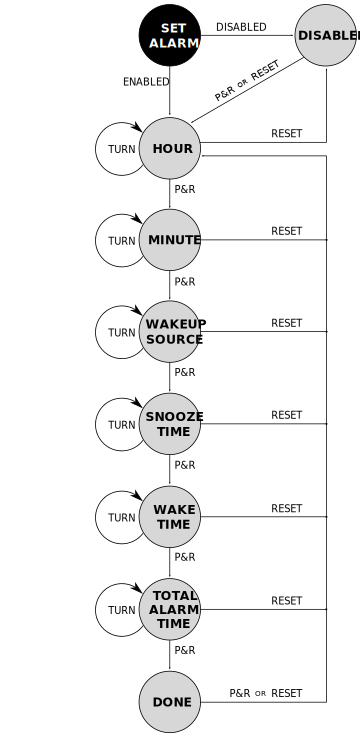
\includegraphics{images/set_alarm_state_diagram.png}
  \caption{Set Alarm - State Diagram}
\end{figure}
